\documentclass[a4paper,UTF8]{article}
\usepackage[scheme = plain]{ctex}
\setCJKmainfont[BoldFont=FandolSong-Bold.otf,ItalicFont=FandolKai-Regular.otf]{FandolSong-Regular.otf}
\setCJKsansfont[BoldFont=FandolHei-Bold.otf]{FandolHei-Regular.otf}
\setCJKmonofont{FandolFang-Regular.otf}

\usepackage{NotesTeX}

\usepackage{graphicx}
\usepackage{circuitikz,tikz}
\usepackage{caption,subcaption}
\usepackage{hyperref}
%\hypersetup{colorlinks,linkcolor = red}
\usepackage{enumitem}
\usepackage[xcolor]{mdframed}
\definecolor{MyBlue}{HTML}{ffeae0}
%\usepackage{tcolorbox}
\theoremstyle{mystyle}{
  \newtheorem{law}{Law}
}
\tcolorboxenvironment{law}{
boxrule=0pt,
boxsep=0pt,
colback={White!90!Cerulean},
enhanced jigsaw,
borderline west={2pt}{0pt}{Cerulean},
sharp corners,
before skip=10pt,
after skip=10pt,
breakable,
}

\usepackage{amsmath,amsthm,amsfonts,amssymb}
%\usepackage{physics,siunitx}
\usepackage{siunitx}

\input macros

\begin{document}

\begin{titlepage}
\newcommand{\HRule}{\rule{\linewidth}{0.5mm}} % Defines a new command for the horizontal lines, change thickness here

\center % Center everything on the page

%----------------------------------------------------------------------------------------
%	HEADING SECTIONS
%----------------------------------------------------------------------------------------

\textsc{\LARGE City University of Hong Kong}\\[1.5cm] % Name of your university/college
\textsc{\Large AP Courses Review Notes}\\[0.5cm] 		% Major heading such as course name
\textsc{\large {AP2212/AP2213}}\\[0.5cm] 						% Minor heading such as course title

%----------------------------------------------------------------------------------------
%	TITLE SECTION
%----------------------------------------------------------------------------------------

\HRule \\[0.4cm]
{ \huge \bfseries  \textsf{(Advanced) Measurement and Instrumentation} }\\[0.4cm] % Title of your document
\rightline{2017--2018 Semester A/B}
\rightline{{\bfseries \textsf{Version 0.2}} }
\HRule \\[1.5cm]

%----------------------------------------------------------------------------------------
%	AUTHOR SECTION
%----------------------------------------------------------------------------------------

\begin{minipage}{0.4\textwidth}
\begin{flushleft} \large
\emph{Author:}\\
 Zezhu \textsc{Wei}
\end{flushleft}
\end{minipage}
~
\begin{minipage}{0.4\textwidth}
\begin{flushright} \large
\emph{Instructor:} \\
Sai Tak \textsc{CHU} % Supervisor's Name
\end{flushright}
\end{minipage}\\[2cm]

% If you don't want a supervisor, uncomment the two lines below and remove the section above
%\Large \emph{Author:}\\
%John \textsc{Smith}\\[3cm] % Your name

%----------------------------------------------------------------------------------------
%	DATE SECTION
%----------------------------------------------------------------------------------------


{\large \today}\\[2cm] % Date, change the \today to a set date if you want to be precise

%----------------------------------------------------------------------------------------
%	LOGO SECTION
%----------------------------------------------------------------------------------------
\vspace{5cm}
%
\includegraphics[scale=0.5]{figures/CityU_full_logo_2015.pdf}\\[1cm] % Include a department/university logo - this will require the graphicx package
%
\includegraphics[scale=0.5]{figures/CityU_logo_2015.eps}\\[1cm] % Include a department/university logo - this will require the graphicx package


%----------------------------------------------------------------------------------------

\vfill % Fill the rest of the page with whitespace
\end{titlepage}

\tableofcontents
\newpage
\part{Measurement System}
\section{Principles of Measurement (01)}
In science, measurement is \emph{the process of estimating or
determining the magnitude of a quantity}, such as length
or mass, relative to a unit of measurement, such as a
meter or a kilogram.

The word measurement is derived from the Greek word ``\textgreek{m'etron}'' m\'etron, 
which means measure.

aggregated.
\subsection{Why Do We Need to Measure?}
\begin{mdframed}

\begin{description}
\item[Consistency] Measurement helps to reduce variation.
\item[Self-Assessment] Measurements can be used to evaluate how well a process is doing, including improvements that have been made.
\item[Process Control] Measurements can be used to identify defects source and process trends, and to determine process efficiency and effectiveness, and the opportunities for improvement.
\end{description}

\end{mdframed}



\subsection{Measurement Unit Systems}

\paragraph{Imperial System (英制单位)}

\paragraph{International System of Units (SI, Syst\`{e}me international)}
Fundamental and Derived Units

\begin{table}[htbp]
\caption{SI base unit}
\centering

\begin{tabular}{lll}
\hline									
Unit	   	&	Macro		 	& 	Symbol			\\
\hline
ampere	 	& \verb|\ampere|	& \si{\ampere}		\\
candela		& \verb|\candela|	& \si{\candela}		\\
kelvin 		& \verb|\kelvin|	& \si{\kelvin}		\\
kilogram 	& \verb|\kilogram| 	& \si{\kilogram}	\\
metre 		& \verb|\metre| 	& \si{\metre}		\\
mole 		& \verb|\mole| 		& \si{\mole}		\\
second 		& \verb|\second| 	& \si{\second}		\\
\hline
\end{tabular}
\end{table}




\begin{table}[htbp]
\caption{SI Prefixes --- Prefixes for Binary Multiples}
\centering

\begin{tabular}{llll}
\hline									
Prefix	   	&	Macro		 	& 	Symbol			& Power\\
\hline
yocto	 	& \verb|\yocto|		& \si{\yocto}		& \num{-24}		\\
zepto		& \verb|\zepto|	& \si{\zepto}		& \num{-24}	\\
atto 		& \verb|\atto|	& \si{\atto}		& \num{-24} \\
femto 		& \verb|\kilogram| 	& \si{\kilogram}	& \num{-24}\\
pico 		& \verb|\metre| 	& \si{\metre}		& \num{-24}\\
nano 		& \verb|\mole| 		& \si{\mole}		& \num{-24}\\
micro 		& \verb|\second| 	& \si{\second}		& \num{-24}\\
milli		& \verb|\second| 	& \si{\second}		& \num{-24}\\
centi		& \verb|\second| 	& \si{\second}		& \num{-24}\\
deci		& \verb|\second| 	& \si{\second}		& \num{-24}\\
\hline
\end{tabular}
\end{table}


\subsection{Measurement Terminology}
\begin{tabular}{|l|l|}
\hline
Metrology 		& Defined as the science of measurement.\\
Instrument 		& Device for recording, measuring or controlling.\\
Instrumentation & The application of instruments for sensing,\\
				& monitoring and measuring.\\
Measurand 		& A physical quantity to be measured.\\
Measurement 	& A quantitative comparison of a measurand \\
				& with a standard (unit).\\
Calibration 	& The process of quantitative comparison \\
				& between a known  standard and the output \\
				& from an instrument for the same quantity. \\
Error 			& Deviation from the true value of the measured variable.\\
\hline
\end{tabular}

\paragraph{Accuracy}
 close the output reading of the measuring instrument to
the correct value.

\paragraph{Precision}
 closeness of one measurement from the other.

\section{Measurement Errors}
Types of Errors
\begin{itemize}
\item System Error (Bias)
\item Random Error
\item Instrumental Errors
\item Environmental Errors
\end{itemize}
Human Error.

68.3\% of the measurements lie
within $\pm 1 \sigma$;
 95.5\% of the measurements lie
within $\pm 2 \sigma$;
 99.7\% of the measurements lie
within $\pm 3 \sigma$.

\subsection{Aggregation of Measurement System Errors}
\begin{description}
\item[Sum or difference]
If two outputs $y$ and $z$ of separate measurement system components
having individual errors of $\Delta y$ and $\Delta z$, respectively, are to be added or
subtracted.
\[
(y \pm \Delta y) + (z \pm \Delta z)
= (y+z) \pm \sqrt{(\Delta y)^2+(\Delta z)^2}
\]
\[
(y \pm \Delta y) \times (z \pm \Delta z)
= (yz) \pm yz
\sqrt{
\left(\frac{\Delta y}{y}\right)^2+\left(\frac{\Delta z}{z}\right)^2}
\]
\[
\frac{y \pm \Delta y}{z \pm \Delta z}
= \frac{y}{z} \pm \frac{y}{z}\sqrt{\left(\frac{\Delta y}{y}\right)^2+\left(\frac{\Delta z}{z}\right)^2}
\]
\end{description}

\section{Elements of Measurement System (02-19)}
A measurement system should have three basic elements each with its own sub-elements:
\begin{enumerate}
\item Transducer (换能器) 

a device that converts energy from one form to another.

\begin{example}[Sensor]
It is the interface between the measurand and 
the measurement system. 
Possible output: Resistance, voltage, 
mechanical deflection, rotation rate. 
It extracts energy from the measured medium 
\emph{ and adds noise to
the signal}.
\end{example}

\item Conditioner
\item Recorder/Display

Analogue type: Pointer type (coil meter);
 Graphical type (plotter, CRO);
 Magnetic type (tape).

 Digital type:
 Computer monitors;
 LED/LCD display.

\subsection{Signal}
A signal is an information-bearing quantity
 Temperature, wind, voltage, current, rotation rate, etc.,
are signals.

 \emph{Analog signal}
 Information is continuously proportional to the measurand
 Measurand (input) and most raw sensor outputs are analog signals.

 \emph{Digital signal}
 Information content varies in discrete steps
 Smaller step sizes yield a digital signal that more closely resembles
the analog signal.
 Output is discrete in both value and time.
\end{enumerate}
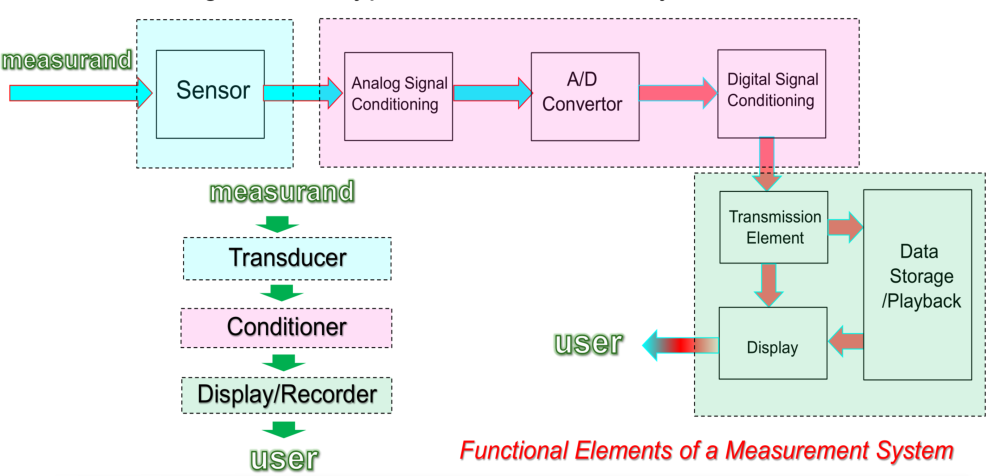
\includegraphics[width=\textwidth]{fig/elements.pdf}

\section{Functional Descriptions of Measuring Instruments (03)}
\subsection{Active and Passive Transducers }
A component whose output energy is supplied entirely
or almost entirely by the input signal.
\paragraph{Active Transducer} 
loud speakers, electrical switches

\paragraph{\textit{Ideal}}
\begin{description}
\item[Linearity] linear relationship between input and output.
\item[High fidelity] Ability to reproduce the measurand without any distortion.
\item[Minimum interference with the measurand] The sensing process does not affect the measurand. Minimum loading or coupling with the measurand.
\item[High stability \& reliability] minimum sensitivity to external effects.
\end{description}

\subsection{Signal conditioning (信号调理)}

Operation performed on signals to convert them to a form suitable for interfacing with other elements in the measurement instrument.

Signal conditioning can be performed with hardware (analog
circuits, springs, ... etc.) or software (algorithm, DSP … etc).

\paragraph{Types of Signal Conditioning}
\begin{enumerate}
\item Linearization:
Provides an output that varies linearly with the measurand
\item Biasing

Apply an offset to the input signal to offset static system error, for
example.
\item Scaling

Increase (amplify) or decrease (attenuate) the magnitude of the
input signal
\item Inverting (逆变器) and Rectifying (整流器)

An invertor inverts the input signal, i.e., putting a negative sign to the input signal.

A rectifier converts an alternating current (AC) input to direct current (DC) output

\item Differentiating and Integrating
\begin{figure}[htbp]
\centering
\caption{Differentiating and Integrating}
\begin{subfigure}{0.45\textwidth}
\begin{circuitikz}[scale = 0.8, transform shape]
  \draw
  (0, 0) node[op amp] (opamp) {}
  (opamp.-) to[C,l=$C$] (-3, 0.5) to [short,-*,l=$V_{\rm in}$] (-3.5,0.5)
  (opamp.-) to[short,*-] ++(0,1) coordinate (leftC)
  to[R,l=$R$] (leftC -| opamp.out)
  to[short,-*] (opamp.out) to [short,-*,l=$V_{\rm out}$] (3,0)
%  (opamp.+) to[short,*-] --(0,1) node[ground]{} to (-1,0)
;\end{circuitikz}
\caption{Differentiation}
\end{subfigure}
%\hfill
\begin{subfigure}{0.45\textwidth}
\begin{circuitikz}[scale = 0.8, transform shape]
  \draw
  (0, 0) node[op amp] (opamp) {}
  (opamp.-) to [R,l=$R$](-3, 0.5) to [short,-*,l=$V_{\rm in}$] (-3.5,0.5)
  (opamp.-) to[short,*-] ++(0,1) coordinate (leftC)
  to [C,l=$C$] (leftC -| opamp.out)
  to[short,-*] (opamp.out) to [short,-*,l=$V_{\rm out}$] (3,0)
%  (opamp.+) to[short,*-] --(0,1) node[ground]{} to (-1,0)
;\end{circuitikz}
\caption{Integrator}
\end{subfigure}
\end{figure}

\item Modulating 

The mixing (adding) of a reference signal (a sinusoidal sign
at some frequency) to the input signal.
It is commonly used in communication, astronomy, and
other fields for detecting, analyzing and transmitting
signals.
\item Filtering 

The process of removing the unwanted component
from the input signal.
e.g.: high-pass, low-pass, band-pass filters.
\end{enumerate}

\subsection{Transfer Function}
The relationship between the input and output signals of a linear 
time-invariant system is called a \textbf{transfer function} ({\tt 传递函数}).\footnote{Conditioning
has a Transfer Function}

\verb|this is transfer function 传递函数|

\emph{Linearity} means that the relationship between the input and the output of the 
system is a linear map: If input $
{\displaystyle x_{1}(t)\,}$  produces response ${\displaystyle y_{1}(t),\,}$, 
and input ${\displaystyle x_{2}(t)\,}$ 
 produces response $y_{2}(t)$, then the scaled and summed input 
${\displaystyle a_{1}x_{1}(t)+a_{2}x_{2}(t)}$  produces the 
scaled and summed response ${\displaystyle a_{1}y_{1}(t)+a_{2}y_{2}(t)}$,  
where ${\displaystyle a_{1}}$  and ${\displaystyle a_{2}}$ are real scalars.

The time-dependent transfer function is often described in two parts, the static part and the dynamic part.

Block Diagrams\\
General Form\\
Cascaded (级联) System\\
Parallel System

\subsubsection{Static Transfer Function}
Describes the input/output relationship when the input is
not changing in time.
It can be presented in the form of equations, tables, or graphs
\subsubsection{Dynamic Transfer Function}
The dynamic transfer function is often represented by a \emph{time-dependent differential equation}.

\paragraph{Response of a First-Order system}
The output is the solution to a first order differential equation.
\[y(t)=y(0)+[y(\infty)-y(0)][1-e^{-t/\tau}]\]
The \emph{time constant $\tau$} is an important parameter of the system.
It provides information on the dynamic behavior of the system.
It is often part of the specification of the sensor/transducer.

 The governing Equation is 
\[
\tau \dv{y(t)}{t} +y(t)=K x(t).
\]

\section{Classification of Instruments}
\begin{enumerate}
\item Deflection-type device
\emph{Less accurate, Faster Response}

The conditioning hardware, such as the spring in the pressure gauge can degrade with time and needs to be calibrated.

It is a direct measurement so the result can be obtained almost instantaneously
\item Null-type device
\emph{More accurate
Slower Response}

It is a direct comparison between the measurand the standard.
It is a relative rather than an absolute measurement.

It requires a comparison step. The time constant is usually slow.
\end{enumerate}



\section{Input/Output Configuration (04-4)}
In lectures 1 and 2, we stated that error exists in any
measurement system.
\begin{itemize}
\item In general, the input signal to the measurement system
consists of both the desired input $I_d$ and the undesired interfering
inputs $I_i$ (noise).
\item The accuracy of the measurement system depends highly on
how one manages the input signal and how to correct these
signals.
\item Besides the desired signal and the undesired interfering signal,
there exist a third signal, \emph{the modifying signal $I_m$, that can cause a
change in the input/output relations for these signals}.
\end{itemize}

\begin{figure}[htbp]
\centering
\caption{Measurement System}
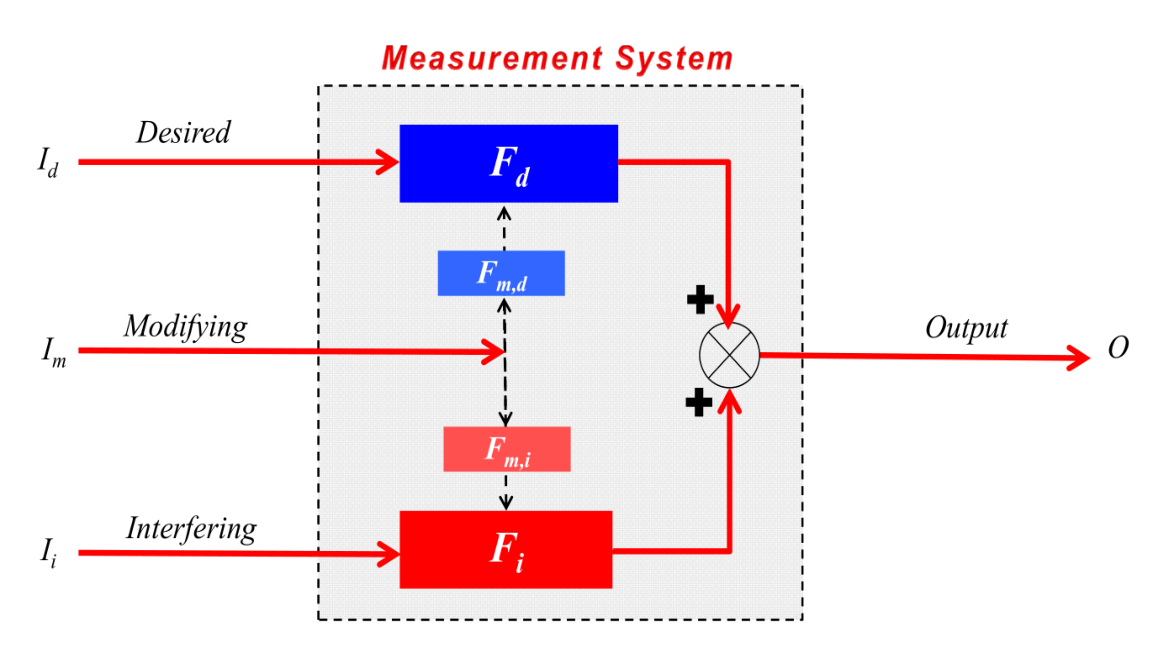
\includegraphics[width=0.9\textwidth]{fig/config}
\end{figure}


$F_d$ \& $F_i$: input/output relations that represent different
concepts depending on the particular input/output
characteristics.

$F_{m,d}$: specific manner in which $I_ m$
affects $F_d$ and $F _i$ , respectively. 
\subsection{Methods of Correction for Interfering and Modifying Inputs}
Methods of Correction:
\begin{description}
\item[Method of Inherent Sensitivity] 
This approach requires that $F_i$ and/or $F_{m,d}$ to be made as
close to zero as possible. Thus effectively eliminates the
effect of $I_i$ and $I_m$ to the output.
\item[Method of Calculated Output Corrections]
This method requires one to estimate the magnitudes of the
interfering and/or modifying inputs and to know
quantitatively how they affect the output. The estimated
value will then be subtracted from the output so as to leave
only the component associated with the desired input.

\item[Method of Opposing Inputs]
This method intentionally introduce additional inputs that
tend to cancel the interfering/modifying inputs.

\item[Method of Signal Filtering]
This method removes the interfering signal if the frequency
of $I_i$ is different from the frequency of $I_d$ .

\item[Method of Negative Feedback (负反馈)]
\[
O=I_d \cdot F_d(I_m)
\]
This method combines a fraction of the output with the
input to reduce the system sensitivity to modifying or
interfering variations.

From the Output, $O=I_d^{adjust}\cdot F_d(I_m)$.
From the input, $I_d^a=I_d-O\cdot F_{feedback}$.
So, 
\[
O=I_d\frac{F_d(I_m)}{1+F_{fb}\cdot F_d(I_m)}
\]

If we select $F_{fb}$ so that $F_{fb}\cdot F_d(I_m) \gg 1$,
\[
O=\frac{I_d}{F_{fb}}
\]
Which is independent of the modifying signal or effects $F_d(I_m)$.

\end{description}



\section{AC Signals (04-17)}
AC signals are commonly used in the field of
electronics, communications and power delivery,
some of the AC signals are:
\begin{description}
\item[Sinusoidal Wave]
$T$ – Period. $f=1/T$, $\omega=2\pi f$, $\theta(t)=\omega t+\phi$,
phase angle $\phi$, $t=0$.

 Amplitude: $y_p = |y| = A$ – Peak Amplitude. $y_pp = 2A$ – Peak-to-Peak Amplitude. Measured between the maximum and
minimum values of the signal. Often it is
the easier measurement to make.

Root-Mean-Square rms: $p_{\rm av}=I_{\rm rms}V_{\rm rms}$.
\[
V_{\rm rms}=\frac{V_p}{\sqrt{2}}
\]
 
\item[Square Wave]
Like the sine waves, square waves are described in terms of
period, frequency and amplitude
\item[Triangular Wave]
\item[Sawtooth Wave]

These signals consist of alternate positive-going and negative
going ramps.

A ramp is a steadily increasing or decreasing of the signal.
\item[Pulse Waveform]
Pulse waveforms is similar to square waves, except that its \emph{minimum
value is above zero}.

Its frequency is referred to as its repetition rate. The time of the pulse
waveform at its maximum (HIGH) is called the \emph{mark}, while when the
pulse waveform at its minimum (LOW) is called the \emph{space}. 
(傳號空號比)
\end{description}

\section{Signal Modulation (04-28)}
Modulation is the process that makes the information
signal (analog or digital) more compatible with the
transmission medium.
We can transmit the same information (signal), such as
voice, over the various communication systems, such as
sonar (sound wave), radio, satellite, microwave and fiber
optics systems.
Although the signal is the same, \emph{the different
communication systems occupy the different parts of the
electromagnetic spectrum}.

\subsection{Spectrum}
The human voice has a range from 50Hz to 7 kHz.
The voice can be described by a frequency spectrum.
The difference between the highest and lowest frequency in a
signal is called its \emph{bandwidth (带宽) BW}.

The type of communication system is
defined by the frequency band it
occupies:\\
  Radio, TV – 50 MHz to 1 GHz\\
  Microwave – 1 GHz to 30 GHz\\
 Fiber Optics – 180 THz to 230 THz

\subsection{Signal Modulation}
The modulated signal that is suitable to be transmitted in
the transmission medium consists\\
 The information signal – also called the \emph{baseband signal}
that carries the message to be sent.\\
 The carrier signal – it has a \emph{higher frequency} than the
baseband signal that depends on the transmission system.

Broadband Transmission (宽带)

 A broadband transmission takes place when a carrier
signal is modulated, amplified and sent to the transmitter,
such as an antenna, for transmission.

\paragraph{Analog Modulation}
 For the transmission of the continuous analog signal
\begin{itemize}
\item Amplitude Modulation (AM) 幅度调制

Carrier amplitude is varied
according to the signal level.

Simple and inexpensive.

Sensitive to the amplitude
variation of the signal due to
noise. It cannot filter out the
noise from the input signal.

\item Frequency Modulation (FM)

More complex and more
expensive.

Less sensitive to the
interference during data
transmission and insensitive
to amplitude variation.

\item Phase Modulation (PM)

\end{itemize}
 \paragraph{Digital Modulation}
 For the transmission of the discrete digital signal
\begin{itemize}
\item Amplitude Shift Keying (ASK) (幅移键控)

Different amplitudes of the carrier represent the level of the
digital signal.
 Susceptible to sudden gain changes and inefficient.
 Very simple and inexpensive

\item Frequency Shift Keying (FSK) (频率偏移调制)

Different frequencies near the carrier frequency represent the
level of the digital signal.
 More reliable and less susceptible to error than ASK.
 Operates at higher frequency
\item Phase Shift Keying (PSK) (相位偏移调制/移相键控)

The phase angle of the carrier signal is shifted to represent
the change of data values.
 The shift can be absolute or relative to the previous bit.
 More complex system but can carry higher capacity.
\end{itemize}


\section{Signal-to-Noise Ratio (05-4)}

\subsection{Noise}
Signal-to-Noise Ratio (SNR) (信噪比) is defined as the ratio between
the noise power versus the signal power and it defines the
detection limit of the system.
\[
{\rm SNR} = \frac{\textrm{Singal Power}}{\text{ Noise Power}}
\]

The unit of measurement for sound level is \textbf{sound pressure level} (s.p.l./声压级) in dB.
\paragraph{Alternate SNR Definition}
In some applications with signal power is not well defined,
such as in imagine processing, it is more convenience to
define SNR as \emph{the ratio between the mean value and the
measured standard deviation $\sigma$}.

\subsection{Types of noises}
\subsubsection{Chemical Noise}
From a source of uncontrollable variable in chemistry.

Changes in pressure, temperature, humidity, external lighting
affecting the collection of the lighting energy from the experiment.

\subsubsection{Instrumentation Noise}
Electrical and/or mechanical noise associated with each
component of instrument.
\begin{description}
\item[Thermal or Johnson Noise]
Caused by thermal agitation of electrons and other charge
carriers in any part of the electronics (resistors, capacitors,
Integrated chips, transistors, wires, connections etc).

The noise increases as the temperature increases and as the
frequency range (bandwidth $\Delta f$) increases.

The noise appears across \emph{all frequencies, thus it is a type of
‘white noise’}.

only be reduce or eliminated by reducing the
temperature of the components.

$v_{\rm rms}\propto \sqrt{T \Delta f}$
\item[Shot Noise (散粒噪声)]
Occurs when electrons or charged particles cross junctions
(different materials, vacuums, solder joints in the circuit board,
etc.)
It is also a \emph{“white noise” that occurs at all frequencies}.
$i_{\rm rms}\propto \sqrt{I e \Delta f}$
\item[Flicker or 1/f noise (闪烁噪声 ,亦称作粉红噪声、 1/f 噪声)]
Pink noise or 1/f noise is a signal or process with a frequency spectrum such that the power spectral density (energy or power per frequency interval) is inversely proportional to the frequency of the signal.\footnote{\url{https://en.wikipedia.org/wiki/Pink_noise}}

Magnitude is inversely proportional to frequency.
Significant at frequencies less than 100 Hz.

\item[Environmental noise]
It varies with location and time.

It is the noise that comes from the environment, our power line, the
rotation of the earth, the radio/TV stations, cell phone signal.. etc.
\end{description}

\paragraph{Noise spectrum}
\begin{center}
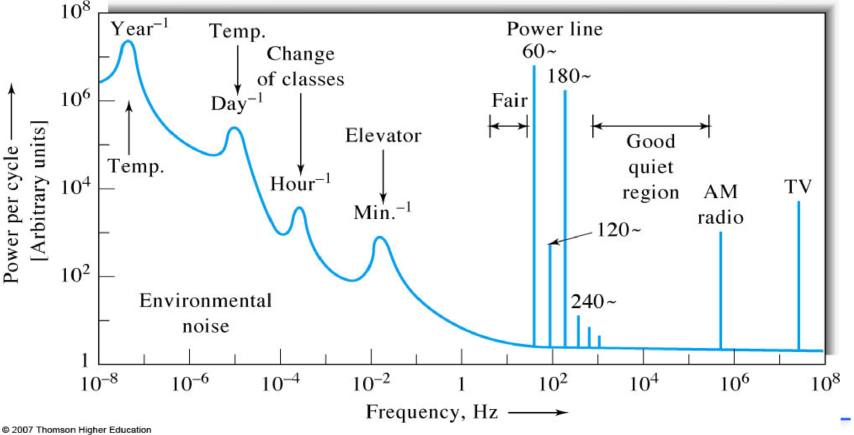
\includegraphics[width=0.9\textwidth]{fig/noise_spec}
\end{center}



\section{Signal-to-Noise Enhancement}
\subsection{Software}
Software methods are based on computer algorithm to extract
the signal from noisy data.
\begin{description}
\item[Ensemble Averaging 总体均值]
Collect multiple measurements at the same time, or taking
multiple measurements per frequency or wavelength.

Calculate the mean signal at each point of the measure
domain.

Since the noise is random, this to purify the signal by
cancellations.
\item[Boxcar Averaging 厢车平均法]
From the single set of data point, the average of the sample
point along with a number of its neighboring points are taken
as its value.

Although the method can be used to reduce the amount of
noise in the measurement, it will also affects the fidelity of the
original signal.

It is often used to study trends in a time series data, most
notably the moving average in financial times series.
\end{description}


\subsection{Hardware}
\begin{description}%[font=$\bullet$\scshape\quad\emph]
\item[Grounding \& Shielding (接地与屏蔽)]

Environmental EM radiation can be reduced by properly
grounding, shielding and reducing the lengths of the conductors
within the instruments.
\item[Analog Filtering]

Low-pass and High-pass analog filters (高通滤波器,低频剪切滤波器) can be utilized to filter
out the unwanted noise from the system.
\item[Modulation]
In this process, low frequency signal from the transducers is
converted to higher frequency, where the \emph{flicker noise} is not as
troublesome.

\item[Signal Chopping (斩波)]

This is a form of modulation, the input signal is converted to a
square-wave form by an electronic or mechanical chopper. The
method essentially converts the input signal into an AC signal
that can be properly amplified.

\item[Lock-in Amplifier (锁相放大器)]

This requires a reference signal that has the same frequency
and phase as the signal to be amplified. A lock-in amplifier is
generally relatively free of noise because only those signals that
are locked-in to the reference signal are amplified. All other
frequencies are rejected by the system.
\end{description}


\section{System Performance Evaluation (05-20)}
The evaluation of a measurement system can be
specified into two parts:
\subsection{Static Performance}
The characteristics associated with the static performance of
a measurement system are:
\begin{itemize}
\item Sensitivity
\item Resolution
\item Precision
\item Linearity
\item Range and threshold
\item Drift – the gradual change of output for a given constant input,
or a change of the sensitivity of the system over time.
\item Hysteresis – the dependence of the system not on its current
input but also on its past input.
\end{itemize}

\subsection{Dynamic Performance --- First order system}
Here we have a few choices that depend on the input signals
\begin{itemize}
\item	Step (transient) response from a step input.
\item	Linear response from a ramp input.
\item	Frequency response from a sinusoidal input.
\end{itemize}
The governing Equation is 
\[
\tau \dv{y(t)}{t} +y(t)=K x(t).
\]
\paragraph{Step or Transient Response}
Input 
\[
x(t)=\begin{cases}
0, & t<0\\
A, & t\geq 0.
\end{cases}
\]
Output
\[
y(t)=\begin{cases}
0, & t<0\\
KA(1-e^{-t/\tau}), & t\geq 0.
\end{cases}
\]

\begin{figure}[htbp]
\centering
\caption{Transient Response}
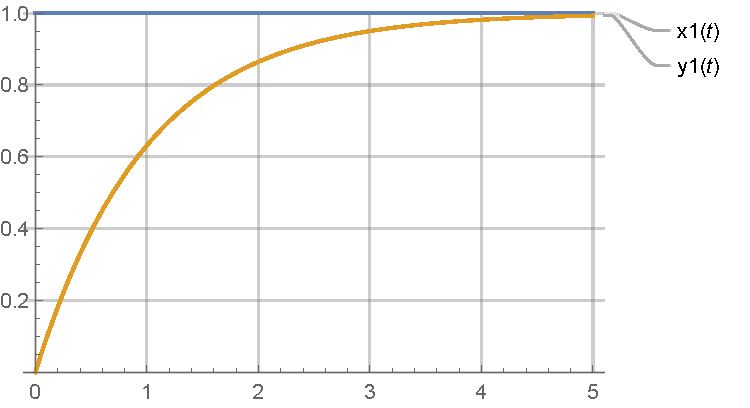
\includegraphics[width=0.7\textwidth]{fig/const_res}
\end{figure}


\paragraph{Linear Response}
Input 
\[
x(t)=At , t>0
\]
Output
\[
y(t)=KA \tau (e^{-t/\tau})+KAt, t>0.
\]
When $t \gg \tau$, $y(t)\sim KA(t-\tau)$.

\begin{figure}[htbp]
\centering
\caption{Linear Response}
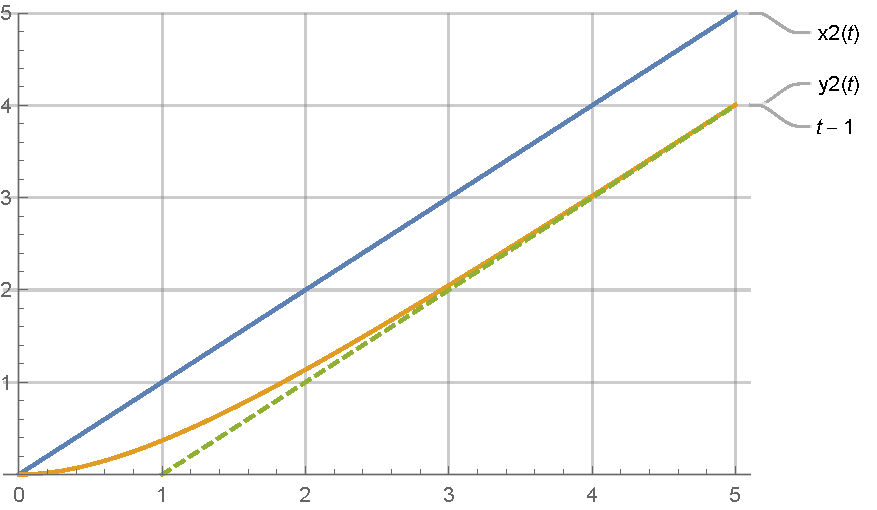
\includegraphics[width=0.7\textwidth]{fig/linear_res}
\end{figure}

\paragraph{Frequency Response} 
Input 
\[
x(t)=A\sin(\omega t), t>0 
\]
Output
\[
y(t)=\frac{KA }{\omega ^2\tau ^2 +1}\left(  \omega\tau  e^{-{t/\tau }}-  \omega\tau  \cos ( \omega t)+\sin ( \omega\tau )\right)
\]
When $t \gg \tau$, $y(t)\sim \frac{KA}{\sqrt{\omega ^2\tau ^2 +1}}\sin(\omega t+\phi)$, where $\phi=-\arctan(\omega \tau)$.

\begin{figure}[htbp]
\centering
\caption{Frequency Response}
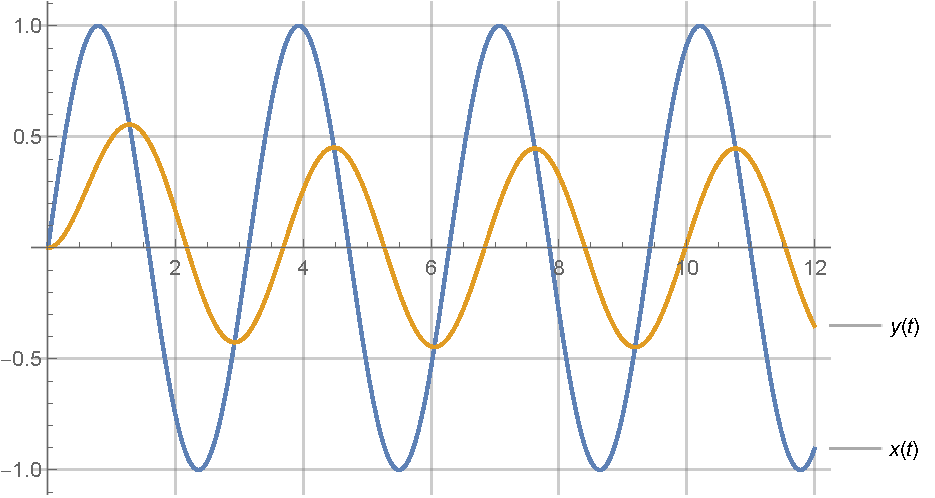
\includegraphics[width=0.75\textwidth]{fig/freq_res}
\end{figure}


\[
\left|\frac{y}{x}\right|=\frac{K}{\sqrt{\omega ^2\tau ^2 +1}}
\]
Output amplitude decreases with increasing
frequency and time constant.
The system cannot react fast enough to catch
up with the input.

\section{Review of Basic Electric Circuits and Components (05-26)}

\section{Dynamic Measurements --- Second Order (06-)}
Spring/mass systems – Load cells, pressure
transducers, accelerometers.
Have damping – dissipate energy.
\[
\frac{1}{\omega_n^2}\dv[2]{y(t)}{t}+\frac{2\zeta}{\omega_n}\dv{y}{t}+y(t)=x(t),
\]
where $\omega_n$ is the \emph{undamped natural frequency}
in rad/s and $\zeta$ (Greek Zeta) is the \emph{damping
factor}.

Laplace Transform allows us to transform the function from
the time domain into a complex frequency domain $s=\sigma+i\omega$.
\[
\mathcal{L}\{f(t)\}= F(s)=\int _{0}^{\infty }f(t)e^{-st}\,dt
\]

\[
\frac{Y(s)}{X(s)}=\frac{\omega_n^2}{s^2+2 \zeta\omega_n s +\omega_n^2}
\]
Note that the denominator of the transfer function is a second
order polynomial of $s$. The roots of this polynomial is called
the \emph{poles} of the transfer function.

Setting the denominator to 0, $s^2+2 \zeta\omega_n+\omega_n^2$.
The poles are
\[
\frac{-2\zeta\omega_n\pm\sqrt{(2\zeta\omega_n)^2-4\omega_n^2}}{2}.
\]

In different cases:
\begin{itemize}
\item $\zeta=0$  undamped
\item $\zeta<1$  under damped
\item $\zeta=1$  critically damped
\item $\zeta>1$  over damped
\end{itemize}

\subsection{Time-response specification}
{\footnotesize\sffamily
More information can be found in \url{http://virtual.cvut.cz/dynlabmods/syscontrol.pdf}, Section 7.3. The archived website is at: \url{https://web.archive.org/web/20141121070451/http://virtual.cvut.cz:80/dynlabmods/syscontrol.pdf} or \url{https://web.archive.org/web/20170812190705/https://www.atp.ruhr-uni-bochum.de/rt1/syscontrol/node57.html}.
}

The rise time $t_r$ is the time required to reach first the steady-state value (100\%). It may also be defined as the time to reach the vicinity of the steady-state value particularly for a response with no overshoot, e.g. the time between 10\% and 90\%. The  rise time $t_{r,50}$ is defined as the time to first reach 50\% of the final value.

The maximum overshoot $M_p$ is the magnitude of the overshoot after the first crossing of the steady-state value (100\%). This value is normally expressed as a percentage of the steady-state value of the controlled variable.

The peak time $t_p$ is the time required to reach the maximum overshoot.
The settling time $t_{\epsilon}$ is the time for the controlled variable first to reach and thereafter remain within a prescribed percentage  of the steady-state value. Common values of  are 2\%, 3\% or 5\%.
\begin{figure}[htbp]
\centering
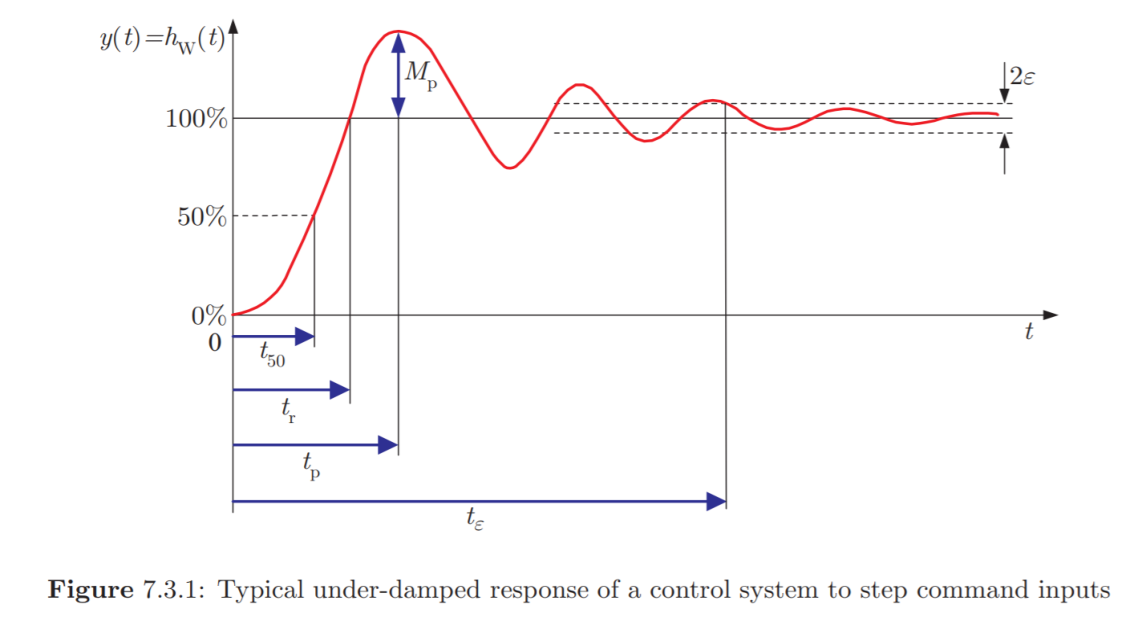
\includegraphics[width=0.9\textwidth]{fig/response}
\end{figure}

\section{Sampling (06-14)}
In order to obtain a picture of a varying quantity we need
to take regular measurements
this process is called sampling (采样)
but how often do we need to sample?

The answer is given by the Nyquist sampling theorem
which says that:
\begin{theorem}[Nyquist–Shannon sampling theorem
\footnote{From: \url{https://en.wikipedia.org/wiki/Nyquist\%E2\%80\%93Shannon_sampling_theorem}} 
奈奎斯特–香农采样定理]
The sampling rate must be greater than \emph{twice the
highest frequency} present in the signal being sampled,
this minimum sampling rate is the \emph{Nyquist rate}.
\end{theorem}


When the sampling rate is below the
Nyquist rate, the original signal
becomes indistinguishable. This is
referred to as aliasing (混叠)\footnote{\url{https://en.wikipedia.org/wiki/Aliasing}}.

If a signal contains unwanted high frequency components
these should be removed before sampling
this is done using a low-pass filter
such a filter is called an \emph{anti-aliasing filter} (抗混叠滤波器).

It is common to sample at about $20\%$ above the Nyquist rate
to allow for imperfect filtering.

\section{Fourier Series (06-18)}
A function can be defined as a series of sines and
cosines\footnote{\url{http://mathworld.wolfram.com/FourierSeries.html}} such that
%\begin{align}
%  s_{N}(x)
%  &=\overbrace {a_{0}} ^{A_{0}}/2+
%  \sum _{n=1}^{N}
%  \left(
%  \overbrace {a_{n}} ^{A_{n}\sin(\phi _{n})} \cos \left({\tfrac {2\pi nx}{P}}\right)		+
%  \overbrace {b_{n}} ^{A_{n}\cos(\phi _{n})} \sin \left({\tfrac {2\pi nx}{P}}\right)
%  \right)\\
%  &=\sum _{n=-N}^{N}c_{n}\cdot e^{i{\tfrac {2\pi nx}{P}}},
%\end{align}
\[
 f(x)=\frac{1}{2}a_0+\sum_{n=1}^\infty a_n \cos(nx)+\sum_{n=1}^\infty b_n \sin(nx), 
\]
where
\begin{align*}
a_0=& \frac{1}{\pi}\int_{-\pi}^{\pi}f(x)\dd{x}	\\
a_n=& \frac{1}{\pi}\int_{-\pi}^{\pi}f(x)\cos(nx)\dd{x}\\
b_n=& \frac{1}{\pi}\int_{-\pi}^{\pi}f(x)\sin(nx)\dd{x}
\end{align*}
and $n=1, 2, 3, \dots$.

\subsection{Exponential Form}
The notion of a Fourier series can also be extended to complex coefficients. Consider a real-valued function $f(x)$. Write
\[
 f(x)=\sum_{n=-\infty}^{\infty}A_n e^{inx}. 
\]
\[
 A_n=\frac{1}{2\pi}\int_{-\pi}^{\pi}f(x)e^{-inx}\dd{x}. 
\]
\[A_n=\begin{cases}
 \frac{1}{2}(a_n+i b_n) &\text{ for } n<0;\\
 \frac{1}{2} a_0 					&\text{ for } n=0; \\
 \frac{1}{2} (a_n-i b_n) 		&\text{ for } n>0.
\end{cases}
\]

\section{Fourier Transform}
For non-periodic signals, we need to consider a periodic
signals as periodic signals with infinite period.

As the period becomes infinite, the corresponding
frequency components form a continuum and the Fourier
series sum becomes an integral.

Instead of looking at the coefficients as a harmonically–
related Fourier series, we'll now look at the \emph{Fourier
transform} which is a \emph{complex valued function} in the
frequency domain.

We will be referring to functions of time and their Fourier
transforms. A signal $f(t)$ and its Fourier transform $g(\omega)$ are
related by the Fourier transform synthesis and analysis
equations

\[
g(\omega)=\int _{-\infty }^{\infty }f(t)\ e^{-j \omega t }\,dt
=\mathcal{F}\{f(t)\},
\]
and
\[
f(t)=\int _{-\infty }^{\infty }g(\omega) \ e^{j \omega t }\dd{\omega}
=\mathcal{F}^{-1}\{g(\omega)\},
\]
where $j^2=-1$.

The transform function $g(\omega)$ can roughly be thought of as
a continuum of the previous coefficients.

\newpage
\part{Electricity and Electronics}
‘Electrical’ is often used to refer to applications that
are concerned with the generation, transmission or use of large amounts of
electrical energy. ‘Electronic’ applications often involve smaller amounts
of power, and in many cases the electrical energy is used to convey information
rather than as a source of power.
\section{DC Circuit}
{\sffamily Read Chapter 12 Resistance and DC Circuits}

\subsection{Kirchhoff's Laws}

\begin{law}[Newton's First Law]
If there is no net force on an object, then its velocity is constant. The object is either at rest (if its velocity is equal to zero), or it moves with constant speed in a single direction.
\end{law}

\subsection{Principle of Superposition}
In any \emph{linear network of resistors}, voltage sources
and current sources, each voltage and current in the
circuit is equal to the algebraic sum of the voltages
or currents that would be present if each source
were to be considered separately.
\begin{remark}

Note that not all circuits are linear, so this principle is
not as universal as Kirchoff's Laws.
For a discussion of superposition principle, you can see:
\url{https://physics.stackexchange.com/questions/165121/is-there-a-formal-proof-for-the-superposition-theorem}
or \url{https://en.wikipedia.org/wiki/Linear_circuit}.
\end{remark}

\subsection{Equivalent Circuits}
%In circuit theory terms, the theorem allows any one-port network to be reduced to 
%a single voltage source and a single impedance. 
\begin{theorem}[Th\'{e}venin's Theorem (戴维南定理、等效电压源定理)
\footnote{The correct one see: \url{http://wps.pearsoned.co.uk/wps/media/objects/1244/1273900/Chap12.ppt}.}]
As far as its appearance from outside is concerned, any \textbf{two terminal
network of resistors and energy sources} can be replaced by a series
combination of an ideal voltage source $V_{\rm OC}$ and a resistor $R$, 
where $V_{\rm OC}$ is the
\textbf{open-circuit voltage} of the network and $R$ is the \textbf{resistance} that would be
measured between the output terminals if \textbf{the energy sources were
removed and replaced by their internal resistance}.
\end{theorem}

\begin{theorem}[Norton's Theorem (诺顿定理、等效电流源定理)]
As far as its appearance from outside is concerned, any two terminal
network of resistors and energy sources can be replaced by a parallel
combination of an ideal current source $I_{\rm SC}$ and a resistor $R$, where 
$I_{\rm SC}$ is the
\textbf{short-circuit current of the network} and $R$ is the voltage that would be
measured between the output terminals if the energy sources were
removed and replaced by their internal resistance.
\end{theorem}

\section{AC circuit}
\subsection{AC signal}
\subsection{capacitors and inductors}

\subsection{Complex representation}

\section{Frequency Response}

\section{Transient response}

\section{Semiconductor Diodes}
A component for which Ohm's law is \emph{not} valid are
called \textbf{nonlinear devices}. They are the basis of
electronic circuits. A diode (二极管) is a type of non-linear 
circuit with two
terminals (hence the name).

\subsection{ideal diode}
An \textbf{ideal diode} is a circuit element that passes
electricity in one direction but not in the opposite.

\begin{circuitikz}
\draw (0,2) to [D*] (0,0);
\end{circuitikz}

In forward bias, resistance $R_D=0$, that is, $V_D=0$ even if 
current $i \neq 0$ (or $i > 0$ with forward direction).
In reverse bias, resistance $R_D=\infty$, that is, current
$i=0$ under whatever voltage like a insulator (or capacitor?). 
In each case, \emph{an ideal diode does not dissipate any power}.


\begin{example}
\end{example}

Semi-condunctor, {\it p-n} junction and semiconductor diode.
\subsection{Currents in {\it p-n} junction}
The $p$-$n$ junction current is 
\begin{equation}
I = I_S \left( \exp \frac{e V}{\eta k T} -1 \right), 
\end{equation}
where e is the electronic charge, $V$ is the applied voltage,
$k$ is Boltzmann constant,
$T$ is the absolute temperature,
$\eta$ is a constant in the range 1 to 2
determined by the junction material (usually $\eta$ = 1).


\begin{definition}[turn-on voltage]
When a semiconductor diode is forward-biased a negligible current will
flow for a small applied voltage, but this increases exponentially as the
voltage is increased. When viewed on a large scale, it appears that the cur-
rent is zero until the voltage reaches a so-called \textbf{turn-on voltage}, and that
as the voltage is increased beyond this point the junction begins to conduct
and the current increases rapidly.
\end{definition}

\subsection{Diode Circuit}

\begin{example}[Half-wave rectifier]
More information at :\url{https://en.wikipedia.org/wiki/Rectifier#Rectifier_output_smoothing}.

(also called a filter, reservoir, or smoothing capacitor 储能电容、滤波电容).
The magnitude of the
ripple (纹波) in the output voltage is affected by the current taken by the load, the
size of the capacitor and the frequency of the incoming signal.

\end{example}


\begin{circuitikz}[scale=0.6]%[/tikz/circuitikz/bipoles/length=1cm]
\draw (-4,2) to 
[V] (-4,8) to 
[short] (4,8) to 
[short] (4,7) to
[D*] (6,5) to 
[short] (10,5) to
[R] (10,0) to
[short] (2,0) to
[short] (2,5) to
[D*] (4,7);  
\draw (-4,2) to
[short] (4,2) to
[short] (4,3) to
[D*] (6,5);
\draw (2,5) to
[D*] (4,3);
\end{circuitikz}

\section{op-amp}
Operational amplifiers are a form of integrated circuit (IC). That is, they
are constructed by integrating a large number of electronic devices into
a single semiconductor component.

\newpage
\part{Sample Problems}

\end{document}